
\chapter{DiLoc - A NN Apporach for Source Localization}
When having enough and suitable data for a problem to solve, one can start building tailorsuited neural networks to address the problem. We aim to build a neural network which aims to map measured EEG signals to localized equivalent current dipoles.
In this chapter, we will provide a comprehensive overview of the feed forward neural network that we have build, reffering to it as \emph{DiLoc}. We will discuss its architecture, parameters and training process. Moreover we will present an alternative approach using a convolutional neural network for the same purpose of source localization.

\section{Machine Learning and Neural Networks}
Machine learning is a field concerned with constructing computer programs that learn from experience, where the utialization of data improves computer performance across various tasks. Within this broad scope, one application could lie in the identification of sources generating abnormal electrical brain signals. By employing specific machine learning algorithms, EEG data can be processed and analyzed to accurately localize the sources responsible for the recorded signals. These algorithms learn from the data and uncover patterns that associate the signals with their corresponding sources, effectively solving the EEG inverse problem. In this chapter, we introduce the field of machine learning and provide an overview of relevant tequniqes for solving our specific EEG inverse problem and its wider implications.

Machine Learning is a subfield of artificial intelligence with the goal of developing algorithms capable of learning from
data automatically" \cite{mehta2019high}. The typical machine learning (ML) problems are addressed using the same three elements. The first element is the dataset $\mathcal{D} = (\textbf{X}, \textbf{y})$ where $\textbf{X}$ commonly is refered to as the design matrix, and consists of independent variables, and $\textbf{y}$ is a vector consisting of dependent variables. Next, we have the model itself, $f(\textbf{x}; \boldsymbol{\theta})$. The ML model can be seen as a function used to predict an output from a vector of input variables, i.e. $f : \textbf{x} \rightarrow y$ of the parameters $\boldsymbol{\theta}$. Finally, the third element, allows us to evaluate how well the model performs on the obervations $\textbf{y}$. This element is known as the cost funtion $\mathcal{C}(\textbf{y}, f(\textbf{X}); \boldsymbol{\theta})$.

\subsection{Neural Networks}
Neural networks are a distinct class of so-called \emph{nonlinear machine learning models} capable of learning tasks by observing examples, without requiring explicit task-specific rules \cite{Hjorth-Jensen2022}. The models mimics the way bilogical neurons trasmit signals, with interconnected nodes known as neurons that communicate through mathematical functions across layers. The layers in neural networks contain an arbitraty number of neurons, where each connection is represented by a weight variable.

The network gathers knowledge by detecting relationships and patterns in data using past experiences known as training examples. These patterns are further updated by the usage of appropriate activation functions and finally presented as the output \cite{nwankpa2018activation}. A neural network consits of many such neurons stacked into layers, with the output of one layer serving as the input for the next. Typically, the neural networks are built up of an input layer, an output layer and layers in between, called hidden layers. In figure \ref{fig:NN_basic_architecture} we have provided the basic architecture of neural networks. Here nodes are depiced as circular shapes, while arrows indicate connections between the nodes.

\begin{figure}
    \centering
    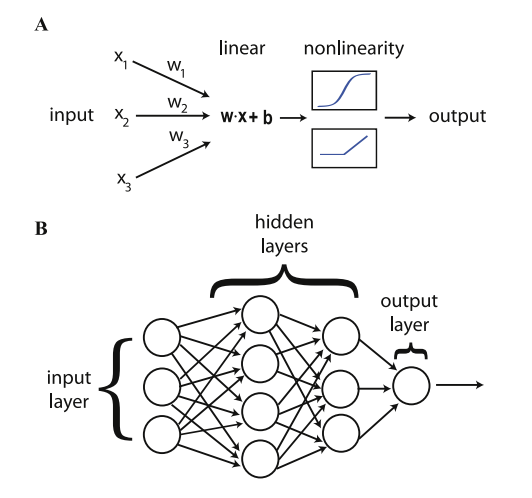
\includegraphics[width=\linewidth]{figures/basic_architecture.png}
    \caption{$\textbf{(A)}$ The fundamental structure of neural networks comprises simplified neuron units that perform a linear operation to assign different weights to inputs, followed by a non-linear activation function.$\textbf{(B)}$ These neuron units are organized into layers, where the output of one layer serves as the input to the subsequent layer, forming a hierarchical arrangement.}
    \label{fig:NN_basic_architecture}
\end{figure}

The behaviour of the human brain has inspired the following simple mathematical model for an artificial neuron:

\begin{equation}
  a = f \left( \Sigma_{i=1}^n w_ix_i \right) ) = f(z)
\label{eq:neuron}
\end{equation}

where $a$ is the output of the neuron, and is the value of the neurons activation function $f$ which has as input a weighted sum of signals $x_i, x_{i+1},...,x_n$ recieved by $n$ other neurons, multiplied with the weights $w_i, w_{i+1}, ..., w_{n}$ and added with bieases $b_i, b_{i+1}, ..., b_{n}$. The exact function $a$ varies depending on the type of non-linearity that exists in the activation function applied to the input of each neuron. However, in almost all cases $a$ can be decomposed into a linear operation that weights the relative importance of the various inputs, and a non-linear transformation $f(z)$. As seen in equation \ref{eq:neuron}, the linear tranformation commonly takes the form of a dot product with a set of neuron-specific weights followed by re-centering with a neuron-specific bias. A more convenient notation for the linear transformation $z^{i}$ then goes as follows:

\begin{equation}
z^{i} = \boldsymbol{w}^{(i)} \cdot \boldsymbol{x} + b^{(i)} = \mathbf{x}^T \cdot \mathbf{w}^{(i)} ,
\label{eq:linear_transformation}
\end{equation}

where $\mathbf{x} = (1, \boldsymbol{x})$ and $\mathbf{w}^i = (b^{(i)}), \boldsymbol{w}^{(i)})$. The full input-output function can be expressed by incorporating this into the non-linear activation function $f_i$, as expressed below.
% TODO: f_i or a_i here?

\begin{equation}
a_i(\mathbf{x}) = f_i(z^{(i)}) .
\label{eq:linear_transformation}
\end{equation}

\section{The creation of DiLoc}
Some basics about DiLoc? How it can be extended blabla..

\subsubsection{Solving The Inverse Problem using Neural Networks}
% notethis
Computational neuroscience is a field that aims to understand the principles underlying information processing in the brain using mathematical and computational tools. The inverse problem in EEG, which involves estimating the location and strength of electrical sources in the brain based on measurements of electrical activity on the scalp, is a key challenge in computational neuroscience. Machine learning techniques, including feedforward neural networks, have been used to address this problem by learning to map the measured EEG signals to estimates of the underlying electrical sources in the brain.

Source localization using machine learning techniques has shown promise for improving the accuracy and efficiency of EEG analysis, and has been applied to a variety of cognitive and clinical applications. For example, machine learning-based source localization has been used to study the neural mechanisms underlying attention, memory, and perception (Wu et al., 2018; Lopes da Silva et al., 2019), as well as to diagnose and monitor neurological disorders such as epilepsy (Safieddine et al., 2019; Shah et al., 2020). These applications demonstrate the potential of machine learning and computational neuroscience to enhance our understanding of the brain and improve clinical outcomes.

Machine learning is a field of computer science that involves using algorithms and statistical models to enable computers to learn from data without being explicitly programmed. One popular type of machine learning algorithm is the feedforward neural network, which is a type of artificial neural network that is often used for tasks such as linear regression. In a feedforward neural network, data is passed through a series of layers of interconnected nodes, or "neurons," which perform mathematical operations to transform the data.

Linear regression is a common machine learning task that involves predicting a continuous quantity, such as the price of a house or the temperature of a city, based on a set of input features. In a feedforward neural network, linear regression can be accomplished by using a single neuron in the output layer of the network that computes a weighted sum of the input features and applies an activation function to produce the predicted output value. The weights on the input features are learned by the network during the training process, which involves adjusting the weights to minimize the difference between the predicted output values and the actual output values in the training data.

Overall, feedforward neural networks are a powerful machine learning tool that can be used to solve a wide range of problems, including linear regression. By adjusting the weights and biases of the neurons in the network during the training process, neural networks can learn to make accurate predictions based on input data, making them a valuable tool for a variety of applications.


\section{The Architecture}
% Dropout 0.5
% Inializer ?
% Include neurons
The development of DiLoc commenced with a deliberate and cautious approach, focusing on simplicity without compromising on accuracy in tackling diverse versions of the inverse problem. As a natural starting point, we adopted a fully connected, feed-forward neural network architecture, which eventually proved to be the most suitable framework for our purposes.

The input layer of DiLoc incorporates Rectified Linear Units (ReLU) as the activation function. This activation function introduces non-linearity into the model, enabling it to capture complex relationships and patterns within the data effectively. For the hidden layers, we employed the hyperbolic tangent (tanh) activation function. This decision was driven by its ability to squash input values into a range between -1 and 1, ensuring a smooth and differentiable transition during backpropagation. Conversely, in the output layer, we opted for a linear transformation without the use of any activation function. This setup allows the neural network to provide direct and unconstrained predictions for the x-, y-, and z-positions of the desired dipole source, as required in our application.

The determination of the number of hidden layers and neurons was carried out through a meticulous trial-and-error process. By experimenting with networks of varying complexities, i.e., small, medium, and large, we ultimately settled on the medium-sized network configuration. This choice, in conjunction with the selected activation functions, yielded the most promising results in terms of prediction accuracies.

The input layer is designed with 231 neurons, corresponding to the number of features in our dataset, i.e. the number of recording electrodes for each sample. Subsequently, the network consists of five hidden layers, comprising 512, 256, 128, 62, and 32 neurons, respectively. Finally, the output layer encompasses the three-dimensional coordinates (x, y, and z) representing the predicted position of the desired dipole source. Figure \ref{fig:FFNN_architecture} visualizes the construction of the fully connected neural network.

\begin{figure}[!htb]
    \centering
    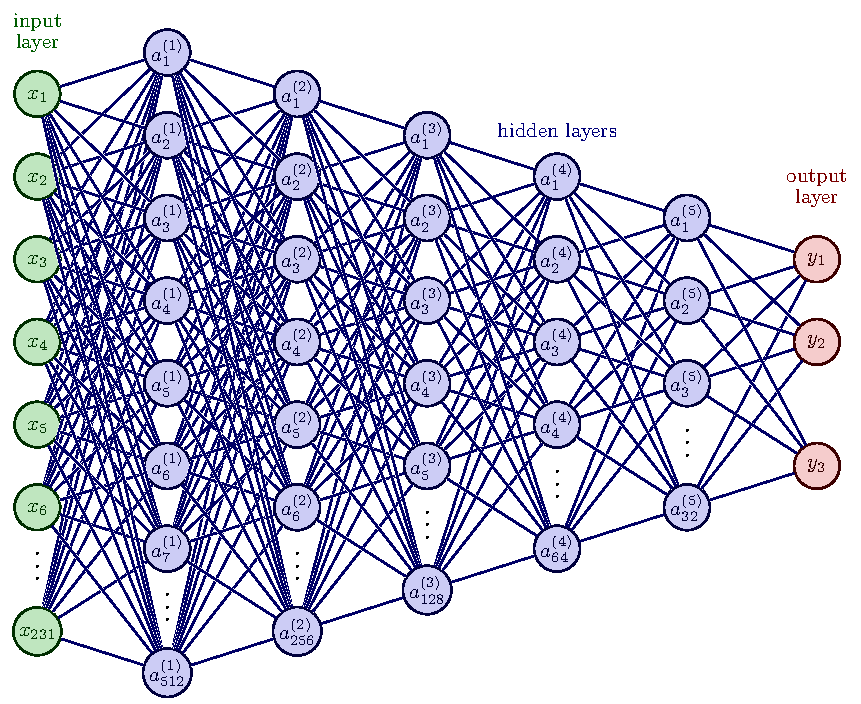
\includegraphics[width=\linewidth]{figures/FFNN_architecture.pdf}
    \caption{Architecture.}
    \label{fig:FFNN_architecture}
\end{figure}


\subsection{Fitting a Machine Learning Model}
Prior to being fed into the DiLoc network for training, the dataset was splittied into distinct segments: the train, validation, and test sets. This partitioning is vital for assessing and optimizing the network's performance. Among the 70 000 samples in the final dataset, 50 000 samples are designated for the train and validation data. To ensure a representative and unbiased allocation, 80 percent of these 50 000 samples are randomly assigned to the training set. This training set serves as the core data that the network utilizes during the training process. The remaining 20 percent of the 50 000 samples form the validation set. This set plays the role in preventing overfitting, the phenomenon where the network becomes excessively attuned to the training data and consequently performs poorly on new data. By independently evaluating the model's performance on the validation set throughout training, we can fine-tune the network's parameters to achieve better generalization to unseen data. Once the network completes its training process, the test set comes into play. Comprising 20 000 samples, the test set serves as the benchmark for assessing the model's ability to generalize and make accurate predictions on new data instances. By adhering to this rigorous train-validation-test data partitioning, we ensure a robust evaluation of the DiLoc model's performance and its capacity to effectively handle real-world scenarios with previously unseen data.

The first step in "fitting" a machine learning model, is to randomly split the dataset $\mathcal{D}$ into train and test sets. This is done in order to make a model compatible with multiple data sets. The size of each set commonly depend on the size of the data set avaible, however a rule of thumb is that the majority of the data are partitioned into the trainng set (e.g., 80$\%$) with the remainder going into the test set \cite{mehta2019high}.

When using the expression "fitting a model" one commonly refer to finding the value of $\boldsymbol{\theta}$ that minimizes a chosen cost function, employing data from the training set. One commonly used cost funtion is the squared error, in which can be written as follows:

\begin{equation}
\text{MSE}(\boldsymbol{\theta}) = \frac{1}{n}
\sum_{i=0}^{n-1}(y_i-\tilde{y}_i)^2 ,
\label{eq:MSE}
%MSE(\textbf{y},\mathbf{\tilde{y}}) =
\end{equation}

where $\boldsymbol{\theta} = \theta_0, \theta_1, ..., \theta_n$ denotes the model parametes, $\tilde{y}_i$ represents the predicted value and $y_i$ is the corresponding true value.

A general expression for any type of cost function can be formulated as follows:

\begin{equation}
C(\theta) = \Sigma^n_{i=0}c_i(\textbf{x}_i, \theta)
\end{equation}

In this expression, $c_i(\textbf{x}_i, \theta)$ represents the cost associated with the $i$-th data point, where $\textbf{x}_i$ represents the input data and $\theta$ denotes the parameter vector. This notation emphasizes the summation over all data points from 1 to $n$, where each data point contributes its own cost to the overall cost function.


\section{Choosing an Optimal Cost Function}
% Include data distribution (min/max)
In the field of machine learning, \emph{cost functions} play a crucial role in evaluating how well models make predictions. These mathematical functions compare predicted outcomes to actual values, resulting in a quantifiable metric known as \emph{loss}. Higher loss values indicate poorer model performance, while lower values reflect more accurate predictions.

Selecting the appropriate cost function is pivotal in addressing machine learning challenges. In regression tasks like ours, the mean squared error (MSE) is a widely used cost function, particularly suitable for linear regression. The MSE is preferred due to its simplicity and continuous measure of model performance during training. It calculates the squared differences between the model's predictions and target values, then takes the mean across the entire dataset:

\begin{equation}
\text{MSE}(\boldsymbol{\theta}) = \frac{1}{N-1}
\sum_{i=0}^{N}(y_i-\tilde{y}_i)^2 ,
\label{eq:MSE}
%MSE(\textbf{y},\mathbf{\tilde{y}}) =
\end{equation}

Here $\boldsymbol{\theta} = \theta_0, \theta_1, ..., \theta_n$ represents the model parametes, $y_i$ stands for the predicted value and $\tilde{y}_i$ is the corresponding true value.

Due to the squaring step in the MSE function, which penalizes larger errors more severely, the trained model is less likely to generate outlier predictions with substantial errors. However, in situations where the model produces a single, highly inaccurate prediction, the squaring effect can significantly amplify the error. Nevertheless, in many practical scenarios, the primary focus is not on these individual outliers, but rather on achieving a well-balanced model that delivers satisfactory performance across the majority of predictions \cite{builtin-ml-loss-functions}.

% include how we do this in our thesis.

In our simulation-driven context, devised to accommodate a spectrum of diverse variations, it's noteworthy that the presence of apparent outliers is not rooted in random fluctuations, but rather indicative of distinct scenarios. As delineated in statistical literature \cite{barnett1994outliers}, an outlier is characterized as an observation that seemingly deviates from the prevailing distribution of a dataset. This departure can be attributed to human or instrumental anomalies in the data acquisition process \cite{zhang2015outlier}. Figure \ref{fig:outliers} vividly depicts the distribution of minimum and maximum EEG observations across individual samples within the dataset. While the majority of data points exhibit values within the range of -1.5 to 3 $\mu$V, a subset extends beyond these bounds. It's crucial to underscore that these data points don't emerge as stochastic errors stemming from the acquisition process. Instead, they intentionally embody distinctive EEG signals that enrich the dataset's representational fidelity within authentic real-world contexts.

\begin{figure}[!htb]
    \centering
    \begin{subfigure}[b]{0.45\linewidth}
        \centering
        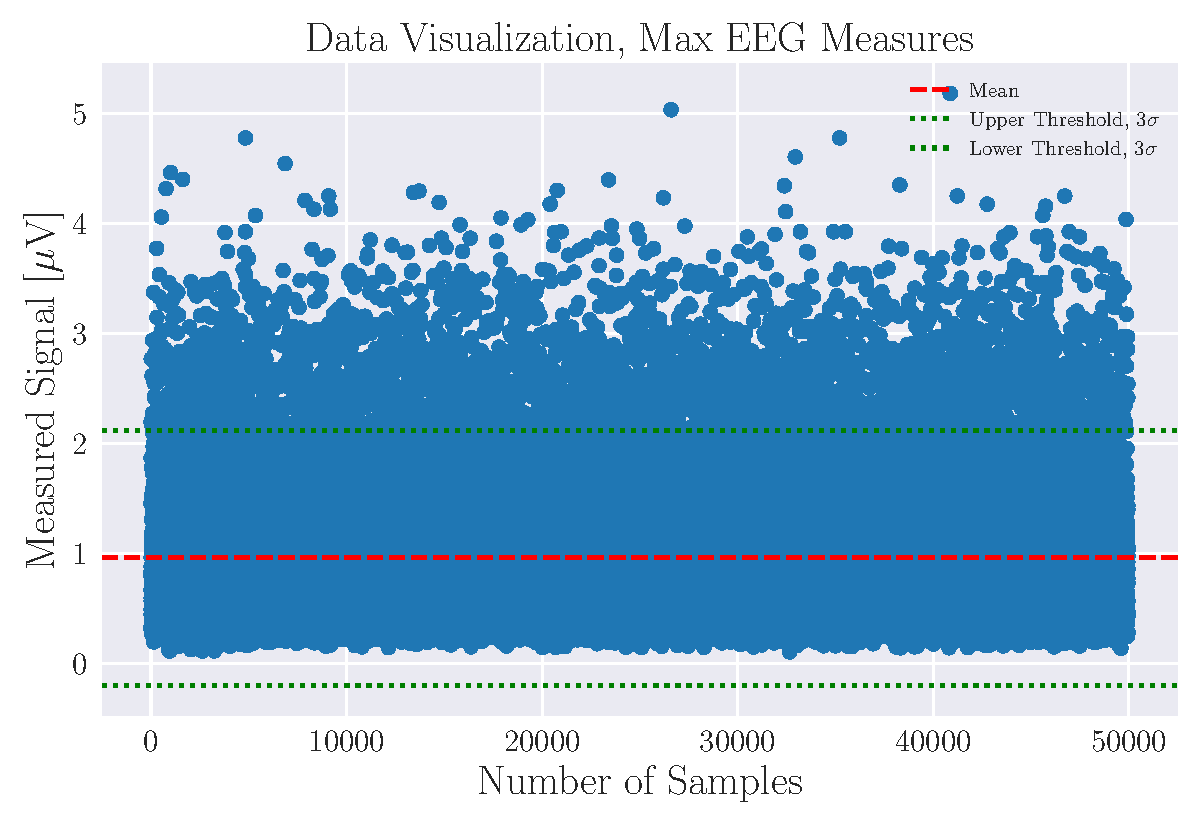
\includegraphics[width=\linewidth]{figures/data_visualization_max.pdf}
    \end{subfigure}
    \hfill
    \begin{subfigure}[b]{0.45\linewidth}
        \centering
        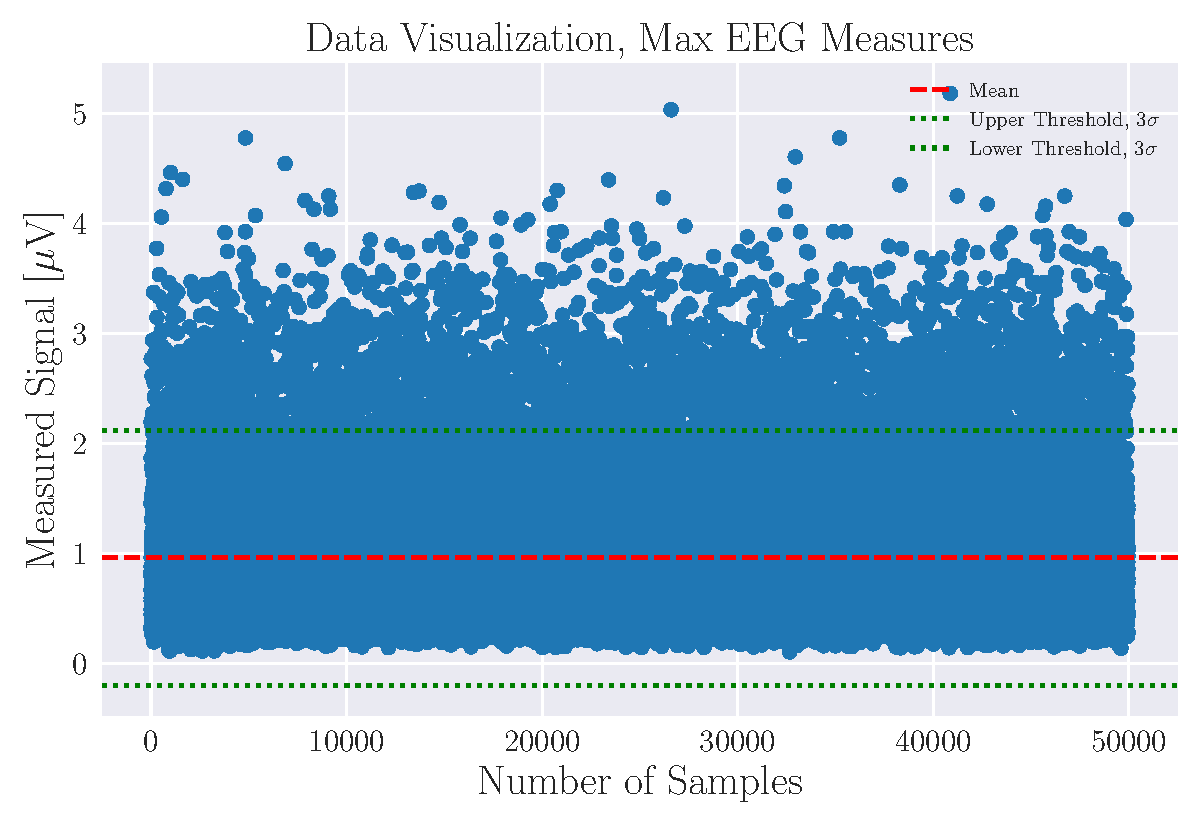
\includegraphics[width=\linewidth]{figures/data_visualization_max.pdf}
    \end{subfigure}
    \caption{\textbf{Visualization of data set.} Both panels visualize the maximum EEG measures for each sample within the data set.}
    \label{fig:outliers}
\end{figure}

When having clear understandings of desired model outcomes, customized cost functions, designed to align precisely with specific objectives may potentially outperform the MSE cost function. Our objective is to create a model that first of all is capable of accurately predicting single dipole posistions, and as extensions also multiple dipole positions, amplitudes of dipole signals and radii of extended dipole populations.  To achieve this, the ideal cost function should minimize the Euclidean distance between target dipole localizations ${\theta}_{x,y,z}$ and true values $\tilde{\theta}_{x,y,z}$:

\begin{equation}
    \text{MED}_{\text{x,y,z}}(\boldsymbol{\theta}) = \frac{1}{n}\sum_{i=0}^{n-1}\sqrt{(\theta_{x,i} - \tilde{\theta}_{x,i})^2 + (\theta_{y,i} - \tilde{\theta}_{y,i})^2 + (\theta_{z,i} - \tilde{\theta}_{z,i})^2},
\label{eq:MED}
\end{equation}

Additionally, the cost function should minimize the absolute error between predicted ${\theta}_{\text{A}}$ and true amplitude $\tilde{\theta}_{\text{A}}$:

\begin{equation}
    \text{MAE}_{\text{A}}(\boldsymbol{\theta}) = \frac{1}{n} \sum_{i=0}^{n-1} \| \theta_{A,i} - \tilde{\theta}_{A,i} \|,
\label{eq:MED}
\end{equation}

Similarly, it should minimize the error between predicted ${\theta}_{\text{r}}$ and true radius$\tilde{\theta}_{\text{r}}$:

\begin{equation}
    \text{MAE}_{\text{r}}(\boldsymbol{\theta}) = \frac{1}{n} \sum_{i=0}^{n-1} \| \theta_{r,i} - \tilde{\theta}_{r,i} \|,
\label{eq:MED}
\end{equation}


Finally, the cost function should minimize the Euclidean distance among a set of $m$ dipoles:

\begin{equation}
\begin{aligned}
    \text{MED}_{\text{x}_1,\text{y}_1,\text{z}_1,\ldots,\text{x}_m,\text{y}_m,\text{z}_m}(\boldsymbol{\theta}) = \\
    &\left( \frac{1}{n}\sum_{i=0}^{n-1}\sqrt{(\theta_{x_1,i} - \tilde{\theta}_{x_1,i})^2 + (\theta_{y_1,i} - \tilde{\theta}_{y_1,i})^2 + (\theta_{z_1,i} - \tilde{\theta}_{z_1,i})^2} \right) + \\
    &\left( \frac{1}{n}\sum_{i=0}^{n-1}\sqrt{(\theta_{x_2,i} - \tilde{\theta}_{x_2,i})^2 + (\theta_{y_2,i} - \tilde{\theta}_{y_2,i})^2 + (\theta_{z_2,i} - \tilde{\theta}_{z_2,i})^2} \right)
    + \ldots + \\
    &\left( \frac{1}{n}\sum_{i=0}^{n-1}\sqrt{(\theta_{x_m,i} - \tilde{\theta}_{x_m,i})^2 + (\theta_{y_m,i} - \tilde{\theta}_{y_m,i})^2 + (\theta_{z_m,i} - \tilde{\theta}_{z_m,i})^2} \right)
\end{aligned}
\label{eq:MED}
\end{equation}

While the built-in MSE cost function compares predicted and target values linearly, the customized cost function should calculate all possible permutations, ensuring the correct combinations are used for loss calculation.

Whereas the standard built-in MSE cost function calculates the mean squared error between each of the target values, we require the customized cost function to map the predictions of each location for the set of dipoles, effectively minimizing the Euclidean distance. Utilizing Python's built-in MSE cost function, the algorithm simply matches predicted locations with the target locations in the order that the vectors have been arranged. However, this technique lacks exploration of other combinations, potentially misleading the network's weight updates if certain accurate locations are paired with non-preferable targets. By enabling the customized cost function to compute all possible permutations, we ensure that the correct target and predicted location values are paired during loss calculation. To achieve this, the cost function calculates all permutations and selects the one yielding the minimum loss.

For all terms within the cost function, comprehensive unit tests have been developed to confirm its intended functionality. Each problem introduced for the network corresponds to a distinct form of the customized cost function:

\begin{equation}
    C(\boldsymbol{\theta}) =
    \begin{cases}
      \begin{array}{l}
      \text{MED}_{\text{x,y,z}}(\boldsymbol{\theta}),
      \end{array} & \text{if } \| \boldsymbol{\theta} \| = 3\\
      \\
      \begin{array}{l}
      \text{MED}_{\text{x,y,z}}(\boldsymbol{\theta}) + MAE_{\text{A}}(\boldsymbol{\theta}),
      \end{array} & \text{if } \| \boldsymbol{\theta} \| = 4\\
      \\
      \begin{array}{l}
      \text{MED}_{\text{x,y,z}}(\boldsymbol{\theta}) + MAE_{\text{A}}(\boldsymbol{\theta}) + MAE_{\text{r}}(\boldsymbol{\theta}),
      \end{array} & \text{if } \| \boldsymbol{\theta} \| = 5\\
      \\
      \text{MED}_{\text{x}_1,\text{y}_1,\text{z}_1,\ldots,\text{x}_m,\text{y}_m,\text{z}_m}(\boldsymbol{\theta}), & \text{otherwise}
    \end{cases}
    \label{eq:cost_function}
\end{equation}

Here, $| \boldsymbol{\theta} |$ signifies the length of the target vector. When $| \boldsymbol{\theta} | = 3$, the simplest problem is considered, where the network predicts the coordinates of a single-point current dipole. If $| \boldsymbol{\theta} | = 4$, the network predicts the x, y, and z-coordinates of a single dipole, in addition to the amplitude of the signal strength. When $| \boldsymbol{\theta} | = 5$, the target vector encompasses all previously mentioned values, along with the size of a current dipole population with radius. Finally, for $| \boldsymbol{\theta} |$ greater than 5, the multiple dipole problem is addressed, where the network predicts the locations for two or more point source dipoles situated at distinct positions within the cortex.

In crafting our customized cost function, it is important to acknowledge that, like the built-in Mean Squared Error (MSE) cost function, our formulation inherently treats all target values equally during the optimization process. In other words, the algorithm assigns the same weight to each target value when striving to reduce the overall loss. This approach ensures that errors of equal percentage magnitude in different target values are treated on a level playing field. Consequently, a 1$\%$ error for one target value is considered as important as a 1$\%$ error for another target value, regardless of the specific range or scale of these values.

It is worth noting that our choice to uniformly weight all target values is an intentional design decision. While alternative approaches, such as assigning different weights to different target values, could have been explored, we prioritize the creation of a balanced model that can accurately predict all facets of our target values. This approach stems from our objective of achieving a comprehensive understanding of EEG signal sources through a holistic and equitable modeling approach.

Moreover, this uniform weighting approach aligns with our broader modeling philosophy, emphasizing the creation of a model that is versatile and adaptable across a spectrum of EEG data variations. Our aim is not only to develop a model capable of accurately predicting target values but also to ensure that its predictive capabilities are unbiased and comprehensive, covering the multifaceted aspects of EEG signal analysis.

In this way, our customized cost function showcases the fusion of machine learning principles with the nuanced requirements of clinical medicine, as we strive to bridge the gap between technical prowess and real-world medical applications.



\subsection {Gradient Descent and Its Variants}
In order to minimize the cost function and find the optimal values for the model parameters, $\boldsymbol{\theta}$, an optimization alorithm is typically employed. One widely used optimization algorithm is gradient descent, which iteratively updates the parameters based on the negative gradient of the cost function.

Gradient Descent (GD) is an iterative optimization algorithm used to locate a local minima of a differentiable function. The core concept of the algorithm is based on the observation that a function $F(\textbf{x})$ will decrease most rapidly if we repeatedly move in one direction opposite to the negative gradient of the function at a given point $\textbf{w}$, $-\nabla F(\textbf{a})$. This means that if

\begin{equation}
\textbf{w}_{n+1} = \textbf{w}_n - \eta\nabla F(\textbf{w}_n)
\end{equation}

for a sufficiently small learning rate $\eta$, we are always moving towars a minimum, since $F(\textbf(w)_n) \ge F(\textbf(w)_{n+1})$ \cite{wiki-gradient-descent}. After each update, the gradient is recalculated for the updated weight vector $\textbf{w}$, and the process is repeated \cite{bishop2006pattern}. Based on this observation, the iterative process begins with an initial guess $x_0$ for a local minimum of the function $F$. It then generates a sequence $\textbf{x}_0, \textbf{x}_1, \textbf{x}_2, ..., \textbf{x}_n$ such that each element in the sequence is upated according to the rule:

\begin{equation}
\textbf{x}_{n+1} = \textbf{x}_{n} - \eta_n\nabla F(\textbf{x}_n), n \ge 0,
\end{equation}

where $\eta_n \ge 0$. The sequence forms what we call a monotonically decreasing sequence:

\begin{equation}
F(\textbf{x}_0) \ge F(\textbf{x}_1) \ge F(\textbf{x}_2) \ge ... \ge F(\textbf{x}_n)
\end{equation}

Hence, with this iterative process, it is hoped that the sequence $(\textbf{x}_n)$ converges to the desired local minimum \cite{wiki-gradient-descent}.

However, it is important to note that the error function in gradient descent is computed based on the training set, so that each step requires that the entire training set, reffered to as the \emph{batch}, is processed in order to evaluate the new gradient. In that sense, gradient descent is generally considered a suboptimal algorithm. This perception aligns with the algorithms sensitivity to the initial condition, $\textbf{w}_0$, and the choice of the learning rate $\eta$. The sensitivity to initial conditions can be explained by the fact that we to a large extent most often deal with high-dimensional, non-convex cost functions with numerous local minima - where the risk of getting stuck in local minimums if the initial guess is not accurate. Additionally, guessing on a too large learning rate may result in overshooting the global minimum, leading to unpredictable behavior, while a too small learning rate increases the number of iterations required to reach a minimum point, thereby increasing computational time. Stochastic gradient descent, however, is a version of gradient descent that has provided useful in practise for training machine learning algorithms on large data sets \cite{bishop2006pattern}.

\subsubsection{Stochastic Gradient Descent}
The method of Stochastic Gradient Descent (SGD) allows us to compute the gradient by randomly selecting subsets of the data at each iteration, rather than using the entire dataset \cite{bishop2006pattern}. The update can be written as:

\begin{equation}
\textbf{w}_{\tau+1} = \textbf{w}_{\tau} - \eta\nabla F_n(\textbf{w}_\tau)
\end{equation}

These smaller subsets taken from the entire dataset are commonly reffered to as mini-batches. In other words, SGD is just like regular GD, except it only looks at one mini-batch for each step. Introducing fluctuation by only taking the gradient on a subset of the data, is beneficial as it enables the algorithm to jump to a new and potentially better local minima, rather that getting stuck in a local minimum point.

\subsubsection{Stochastic Gradient Descent with Momentum}
% TODO: explain why. some more figrues
Splitting the dataset into mini-batches, as done with SGD, naturally reduces the calculation time. However, adding \emph{momentum}, to the algorithm, not only leads to faster converging, due to stronger acceleration of the gradient vectors in the relevant directions, but also improves the algorithms sensitivity to initial guess of the learning rate $\eta$. The momentum can be understood as a memory of the direction of the movement in parameter space, which is done by adding a fraction $\gamma$ of the weight vector of the past time step to the current weight vector:

\begin{equation}
\textbf{v}_{\tau} = \gamma\textbf{v}_{\tau-1} - \eta\nabla F_n(\textbf{w}_{\tau})
\end{equation}

\begin{equation}
\textbf{w}_{\tau} = \textbf{w}_{\tau-1} + \textbf{v}_{\tau}
\end{equation}

Here, $\textbf{w}{\tau}$ represents the updated weight vector at iteration $\tau$, $\textbf{w}_{\tau-1}$ is the previous weight vector, $\textbf{v}_{\tau}$ is the updated momentum vector at iteration $\tau$, $\gamma$ is the momentum coefficient, $\eta$ is the learning rate, and $\nabla F_n(\textbf{w}_{\tau})$ is the gradient of the cost function $F_n$ computed on the mini-batch.


\section{Training the DiLoc Network}
To train the DiLoc network efficiently, several key techniques are employed, including stochastic gradient descent (SGD), mean squared error (MSE) as the cost function, learning rate scheduling, and L1 and L2 regularization. Detailed explanations of these techniques can be found in the Chapter 3.

The objective during training is to find the optimal parameters $\beta$ that minimize the cost function. The cost function represents the discrepancy between the network's predictions and the actual target values. By iteratively updating the parameters to minimize the cost function, the network fine-tunes its internal representations to make more accurate predictions. MSE is chosen as the cost function for the DiLoc network, as it provides a smooth and continuous measure of the model's performance during training, penalizing larger errors more heavily.

% Include why we went for batch size 32 and mom = 0.35 (instead of 0.9)
Optimizers play a crucial role in reducing the network's loss and providing accurate results. In this case, SGD with momentum is utilized as the network's optimizer. SGD with momentum enhances the sensitivity of the network to initialized weights and provides fast convergence. The algorithm uses mini-batches of size 32, introducing fluctuation to the data and preventing the network from getting stuck in local minima or saddle points. The momentum hyperparameter, set to 0.35 in this context, helps reduce high variances in the optimization process and accelerates convergence towards the right direction, leading to faster training.

To improve the training process further, learning rate scheduling is employed. This technique adjusts the learning rate over time, allowing the network to take larger steps in the early stages and gradually decrease the learning rate as it approaches convergence. The initial learning rate is set to 0.001, and is further decreased, which provides balance between rapid convergence in the initial phases and fine-tuning towards the end.

Additionally, L1 and L2 regularization techniques are incorporated as optional parameters into the DiLoc network. These regularization methods help prevent overfitting and improve generalization to unseen data. By adding penalty terms to the cost function, L1 and L2 regularization encourage the model to favor simpler and more generalizable solutions.

After the DiLoc network is fully trained on the training dataset, it has learned the optimal parameters to make accurate predictions. The model's performance is evaluated using a separate test dataset, which the network has not seen during training. This test data provides an unbiased assessment of the model's accuracy and its generalization capabilities to unseen data.

In the upcoming chapters, we will present different approaches to the inverse problem and showcase the performance of the DiLoc network across these approaches. The evaluation results will demonstrate the effectiveness and utility of the trained model in solving the localization task for various scenarios.


\subsection{Activation functions}
Without activation functions, a neural network would essentially be a linear model, capable only of representing linear relationships between inputs and outputs. While the linear transformations occurs within individual neurons through the weighted sum of inputs, the introduction of non-linear activation functions allows the networks to capture complex relationships and patterns. With other words, activcation functions are important components of neural networks, that help the network learn by making sense of non-linear and complex mappings between input- and corresponding output values. The functions are applied at every node in the hidden layers and the output layer \cite{choose_activation_function}.

Activation functions in neural networks draw inspiration from the behavior of neurons in the brain. Similar to how neurons respond to incoming electrical signals, activation functions determine whether a neuron in a neural network should be activated or not based on the strength of the input. If the input exceeds a certain threshold, the neuron "fires" or becomes activated, otherwise it remains inactive \cite{analyticsvidhya_activationfunctions}. By introducing nonlinearity, activation functions enable neural networks to model complex, nonlinear relationships in data.


\subsubsection{Sigmoid}
The sigmoid activation function is one of the more biologically plausible as the output of inactivated neurons returns zero \cite{Jensen2022}. More precised it is a logistic mathematic function meaning that it maps its input to a value between 0 and 1:

\begin{equation}
  f(x) = \frac{1}{1 + e^{-x}}
\label{eq:Sigmoid}
\end{equation}

The function is continuous, ensuring that it is differentiable at every point. This differentiability property plays a crucial role in effective computation of the derivative during the process of backpropagation, as we will explore in more detail in the subsequent sections of this chapter.

The sigmoid activation function maps large negative values towards 0 and large positive values towards 1. Thus, the activation function is commonly utilized in the output layers of neural networks, particularly in classification problems where the desired output can be interpreted as a class label. As we can see from figure \ref{fig:sigmoid}, the function return 0.5 for an input eqal to 0. Due to this, the value 0.5 can be seen as a therhold value which decides wether the input value belongs to what type of two classes.

\begin{figure}
    \centering
    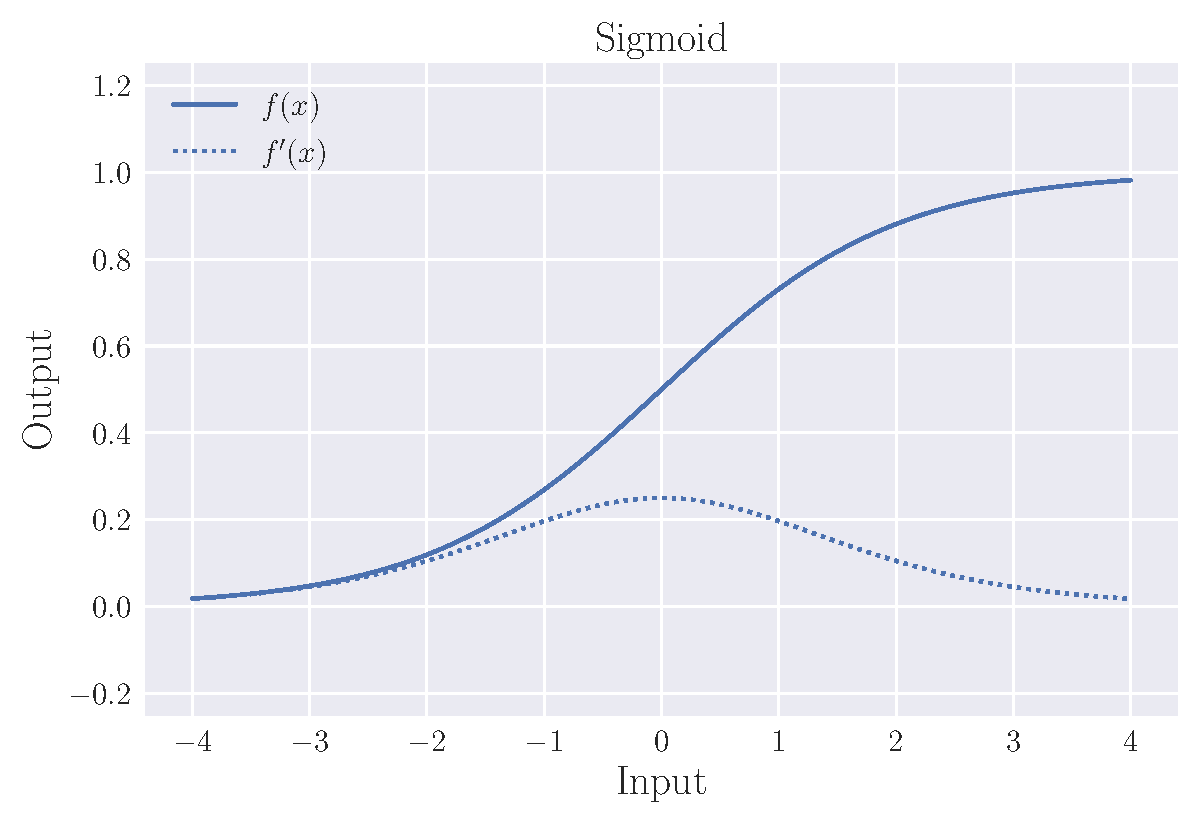
\includegraphics[width=\linewidth]{figures/Sigmoid.pdf}
    \caption{Sigmoid activation function.}
    \label{fig:sigmoid}
\end{figure}

\subsubsection{Hyperbolic Tengent}
The hyperbolic tangent (Tanh) is similar to the Sigmoid function, as it is continuos and differentiable at all points:

\begin{equation}
  f(x) = \frac{{e^x - e^{-x}}}{{e^x + e^{-x}}}
\label{eq:I}
\end{equation}

However, compared to the Sigmoid function, the gradient of Tanh is steeper. Moreover this activation function maps its input to a value ranging between -1 and 1 as seen in Figure \ref{fig:Tanh}

Even though Sigmoid has its advantages, it has been shown that the Hyperbolic tangent performs better than the Sigmoid when approaching complex machine learning problems. The reasons for this will be discussed in later in this chapter.

\begin{figure}
    \centering
    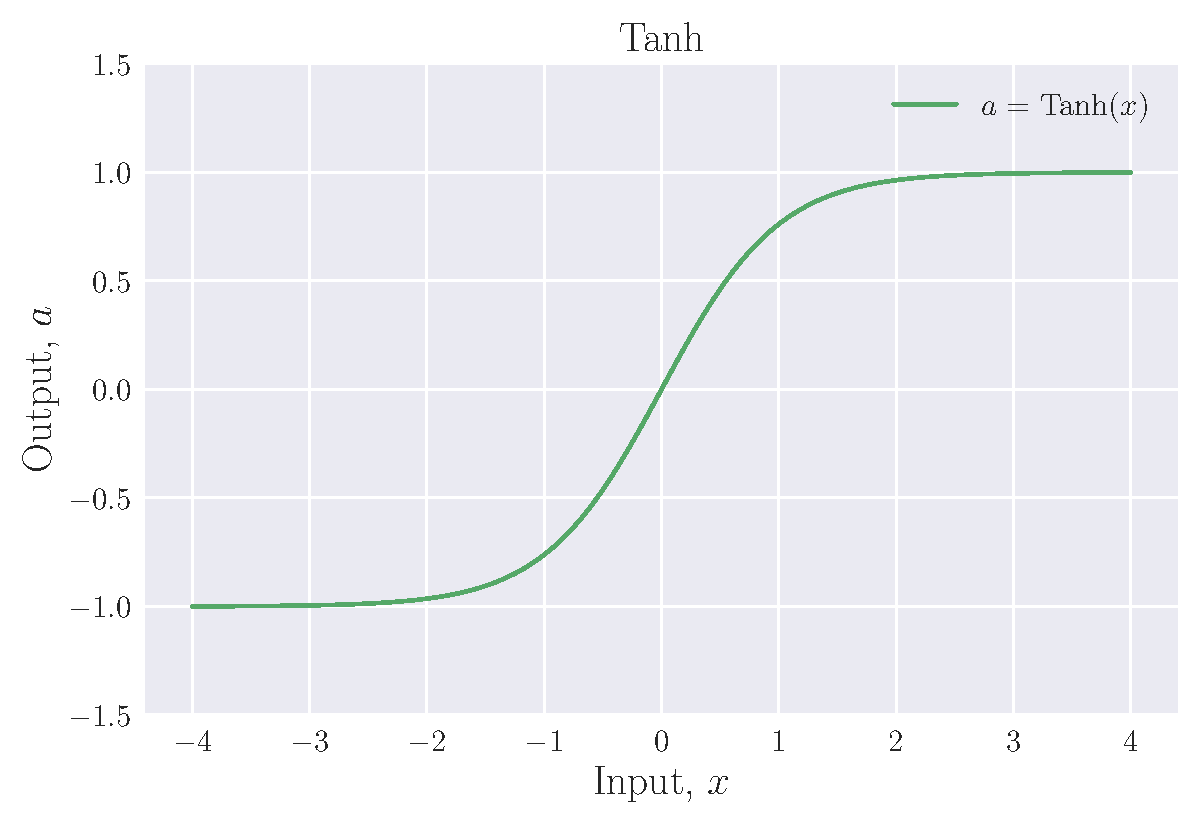
\includegraphics[width=\linewidth]{figures/Tanh.pdf}
    \caption{Hyperbolig tangent activation function.}
    \label{fig:Tanh}
\end{figure}

\subsubsection{Rectified Linear Unit}
The Rectified Linear Unit (ReLU) activation function is widely recognized for its speed, high performance, and generalization capabilities \cite{wandb_activation_functions}. Compared to the Sigmoid and Hyperbolic Tangent functions, ReLU may seem relatively simple, which contributes to its computational efficiency. The function can be mathematically defined as:

\begin{equation}
    f(x) = \begin{cases}
        x, & \text{if } x > 0 \\
        0, & \text{otherwise}
    \end{cases}
\label{eq:ReLU}
\end{equation}

From Figure \ref{fig:ReLU}, it is evident that ReLU retains the input value when the input is greater than zero, and outputs zero for negative inputs. This sparse nature of the activation function enhances computational efficiency as only a few neurons are activated at any given time.

% Include some of this? However, negative values have a derivative of 0, causing potential dead neurons. Leaky ReLU addresses this issue.

\begin{figure}
    \centering
    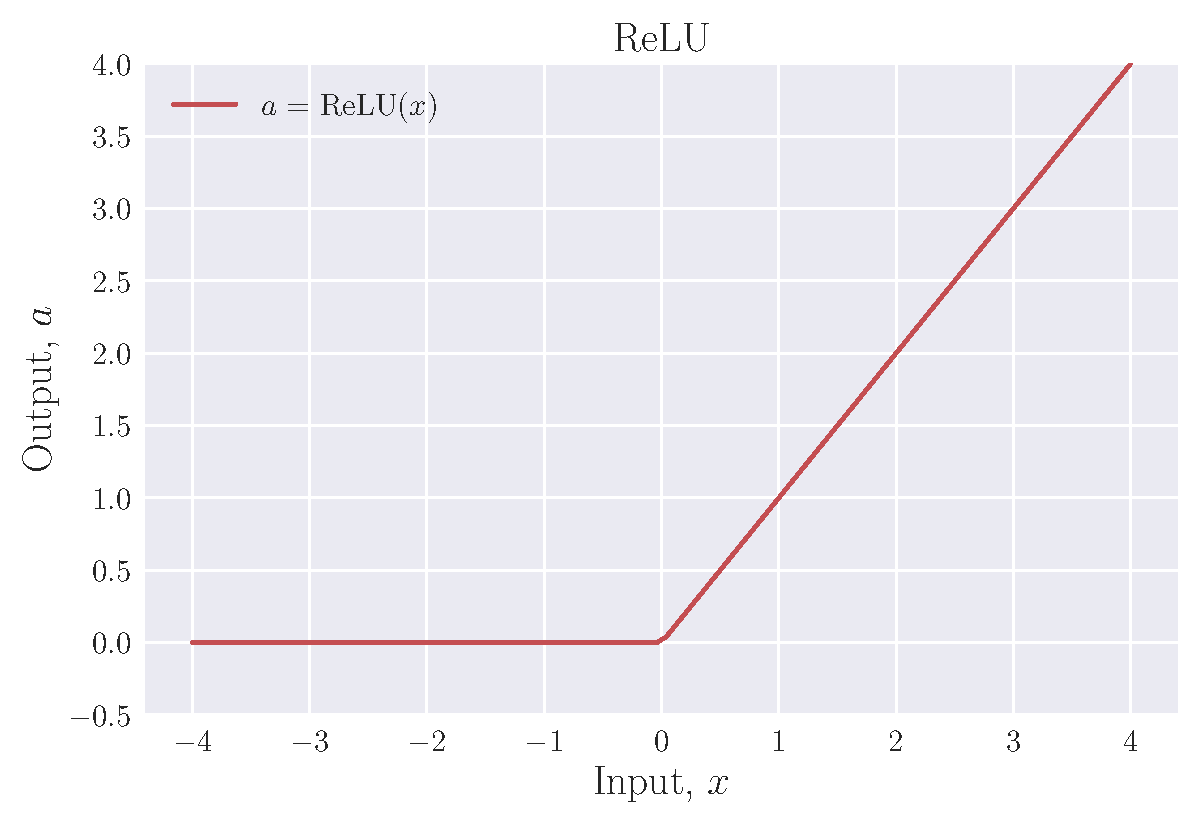
\includegraphics[width=\linewidth]{figures/ReLU.pdf}
    \caption{ReLU tangent activation function.}
    \label{fig:ReLU}
\end{figure}


\subsubsection{Back propagation algorithm}
The back propagation algorithm is a fundamental tequniqe used in nenural networks in order to adjust the weights for the purpose of minimizing the cost function. To explain the implementation details of this technique, we follow the guidance provided in the book 'A high-bias, low-variance introduction to machine learning for physicists' (Pankaj Mehta, et al., 2019) as it offers a comprehensive treatment of the topic. The back propogation tequniqe leverages the chain rule from calculus to compute gradients for weight adjustments and can be summarized using four equations.

Before Introducing the equations, Mehta et al. establish some useful notation. They start by concidering a total of $L$ layers within the neural network, with each layer identified by an idec $l$ ranging from 1 to $L$. For each layer, they further assign weights denoted as $\mathbf{w}^l_{ik}$, which represent the connections between the $k$-th neuron in the previous layer, $l-1$, and the $i$-th neuron in the current layer, $l$. Additionally, they assign a bias value $b^l_i$ to each neuron in the current layer.

The first eqation setting up the algorithm is the definition of the error $\delta_i^l$ of the $i$-th neuron in the $l$-th layer:

\begin{equation}
    \delta_i^l = \frac{\partial C}{\partial(z_i^l)},
\label{eq:I}
\end{equation}
where $(z)$ denotes the weighted input. This equation can be thought of as the change to the cost function by increasing $z_i^L$ infinitesimally. The cost function quantifies the discrepancy between the network's output and the target data. If the error $\delta_i^L$ is large, it indicates that the cost function has not yet reached its minimum.

The error $\delta^l_i$ can also be interpreted as the partial derivative of the cost function with respect to the bias $b^l_i$. This gives us the analogously defined error:

\begin{equation}
    \delta_i^l = \frac{\partial C}{\partial(z_i^l)} = \frac{\partial C}{\partial(b_i^l)}\frac{\partial C}{\partial(z_i^l)} = \frac{\partial C}{\partial(b_i^l)}
\label{eq:II}
\end{equation}
where it in the last line has been used that the derivative of the activation function with respect to its input evaluates to 1, $\partial b^l_i / \partial z_i^l = 1$, meaning that the rate of change of the activation function does not depend on the specific value of the weighted input $z_i^l$.

By applying the chain rule, we can express the error $\delta_i^l$ in Equation \ref{eq:I} in terms of the equations for layer $l+1$. This forms the basis of the third equation used in the backpropagation algorithm:

\begin{align}
\delta_i^l = \frac{\partial C}{\partial z^l_{i}}
&= \sum_j \frac{\partial C}{\partial z_j^{l+1}}\frac{\partial z_j^{l+1}}{\partial z_i^l} \nonumber \\
&= \sum_j \delta_j^{l+1} \frac{\partial z_j^{l+1}}{\partial z_i^l} \nonumber \\
&= \sum_j \delta_j^{l+1}w_{ij}^{l+1}f'(z_i^l) \label{eq:III}
\end{align}

Finally the last equation of the four back propagation equations the derivative of the cost function in terms of the weights:

\begin{equation}
    \frac{\partial C}{\partial w^l_{ij}} = \delta_i^l a_j^{l-1}
\label{eq:IV}
\end{equation}

With these four equations in hand we can now calculate the gradient of the cost function, starting from the output layer, and calculating the error of each layer backwards. We then have a way of adjusting all the weights and biases to better fit the target data. The back propagation algorithm then goes as follows:

\begin{enumerate}
  \item \textbf{Activation at input layer:} calculate the activations $a_i^1$ of all the neurons in the input layer.
  \item \textbf{Feed forward:} starting with the first layer, utilize the feed-forward algorithm through \ref{eq:FFNN} to compute $z^{l}$ and $a^{l}$ for each subsequent layer.
  \item \textbf{Error at top layer:} calculate the error of the top layer using equation \ref{eq:I}. This requires to know the expression for the derivative of both the cost function $C(\boldsymbol{W}) = C(\boldsymbol{a}^L)$ and the activation function $f(z)$.
  \item \textbf{"Backpropagate" the error:} use equation \ref{eq:III} to propagate the error backwards and calculate $\delta_j^l$ for all layers.
  \item \textbf{Calculate gradient:} use equation \ref{eq:II} and \ref{eq:IV} to calculate $\frac{\partial C}{\partial z^l_{i}}$ and $\frac{\partial C}{\partial w^l_{ij}} = \delta_i^l a_j^{l-1}$. \newline
  \item \textbf{Update weights and biases:} \\[2pt] $w^l_{jk}=w^l_{jk}-\eta\delta^l_ja^{l-1}_k$ \\[2pt] $b_j^l = b_j^l - \eta \delta_j^l$
\end{enumerate}

\subsubsection{Initialization of weights and biases}

Sigmoid is usually not utilized in the hidden layers of networks due to vanishing or exploding gradient problems. This term is used in scenarios where the gradient becomes very small, making the optimization process slower and less effective. Such a problem hinders the convergence of the network and makes it challenging, if not impossible, for the network to learn meaningful representations from the data. Looking at the derivative of the function shown in Figure \ref{fig:sigmoid}, we see that we encounter such scenarios when the input value is considerably small or large.

An important advantage of using the hyperbolic tangent function over the sigmoid function is that the tanh function is centered around zero. This makes the optimization process much easier as it ensures that the gradients calculated during backpropagation have both positive and negative values, resulting in more balanced weight updates. This, in turn, might lead to faster convergence and more efficient optimization.





\subsubsection{Feed Forward Neural Networks}
The feedforward neural network (FFNN) was one of the first artificial neural network to be adopted and is yet today an important algorithm used in machine learning. The feed forward neural network is the simplest form of neural network, as information is only processed forward, from the input nodes, through the hidden nodes and to the output nodes \cite{Hjorth-Jensen2022}.


\subsubsection{Convolutional Neural Networks}
Convolutional neural networks (CNNs) is an other variant of FFNNs that have drawen inspiration from the functioning of the visual cortex of the brain. In the visual cortex, individual neurons exhibit selective responses to stimuli within small sub-regions of the visual field, known as receptive fields. This property allows the neurons to effectively exploit the spatially local correlations present in natural images. Mathematically, the response of each neuron can be approximated using a convolution operation \cite{Hjorth-Jensen2022}.

% TODO: check sources
CNNs mimic the behavior of visual cortex neurons by utializing a specific connectivity pattern between nodes in adjacent layers. Unlike fully contected FFNNs, where each node connects to all nodes in the preceding layer, CNNs  local connectivity. In other words, each node in a convolutional layer is only connected to a subset of nodes in the previous layer. Typically, CNNs consist of multiple convolutional layers that learn local features from the input data. These layers are followed by a fully connected layer that combines the learned local information to produce the final outputs. CNNs find wide applications in image and video recognition tasks \cite{Hjorth-Jensen2022}.

\subsection{Neural Networks}
Artificial Neural Networks are computational systems that can learn to perform tasks by considering examples, generally without being programmed with any task-specific rules \cite{101}.

The biological neural networks of animal brains, wherein neurons interact by sending signals in the form of mathematical functions between layers, has inspired a simple model for an artificial neuron:

\begin{equation}
    a = f \left( \Sigma_{i=1}^n w_ix_i + b_i\right ) = f(z)
    \label{eq:NN}
\end{equation}

where the output $a$ of the neuron is the value of its activation function $f$, which as input has the sum of signals $x_i, x_{i+1}, ..., x_n$ received by $n$ other neurons, multiplied with the weights $w_i, w_{i+1}, ..., w_n$ and added with biases.

Most artificial neural networks consists of an input layer, an output layer and layers in between, called hidden layers. The layers consists of an arbitrary number of neurons, also referred to as nodes. The connection between two nodes is associated with a weight variable $w$, that weights the importance of various inputs. A more convenient notation for the activation function is:

\begin{equation}
    a_i(\boldsymbol{x}) = f_i(z^{(i)}) = f_i(\boldsymbol{w^{i}}\cdot \boldsymbol{x} + b^{i})
\label{eq:NN_vec}
\end{equation}

where $\boldsymbol{w}^{(i)} = (w_1^{(i)}, w_2^{(i)}, ..., w_n^{(i)})$ and $b^{(i)}$ are the neuron-specific weights and biases respectively. The bias is normally needed in case of zero activation weights or inputs \cite{101}.

\section{Feed-Forward Neural Network Approach for localizing single dipole sources}
The feedforward neural network (FFNN) was one of the first artificial neural network to be adopted and is yet today an important algorithm used in machine learning. The feed forward neural network is the simplest form of neural network, as information is only processed forward, from the input nodes, through the hidden nodes and to the output nodes.


% \subsection{DiLoc}
% The FFNN that are trained to solve the inverse problem of ours has an input layer of 231 neurons, corresponding to the M = 231 electrode measures of the potentials. The input layer is followed by three hidden layers with 120, 84 and 16 hidden neurons, respectively. When the aim is to estimate the localization of the current dipole, \emph{only}, the final output layer holds the predicted x-, y- and z- position of the desired dipole source.  However, if the interest lies in determining the size of the dipole population, an alternative output layer is incorporated in the network architecture providing the radius of the dipole(s), in addition to the location coordinates. This enables the model to provide a more comprehensive understanding of the dipole source(s) being analyzed.
%
% \begin{figure}
%   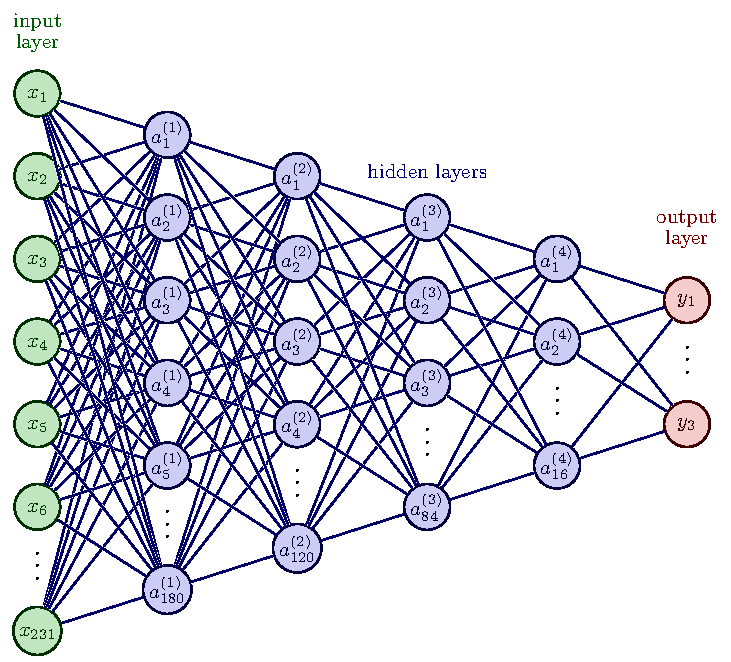
\includegraphics[width=\linewidth]{figures/NN_simple_dipole_architecture.pdf}
%   \caption{A caption here is needed.}
%   \label{fig:NN_architecture.png}
% \end{figure}

\subsection{Validation accuracy}
In Figure \ref{fig:single_dipole_accuracy} we have provided the validation accuray, using mean squared error (MSE) and the coefficient of determination (R2-score).

The expression for MSE when predicting the x-, y- and z-coordinate, goes as follows:

\begin{equation}
MSE(\hat{y},\hat{\tilde{y}}) = \frac{1}{n}
\sum_{i=1}^{n}(y_i-\tilde{y}_i)^2 \\
= \frac{1}{3}\sum_{i=1}^{3}((x-\tilde{x})^2 + (y-\tilde{y})^2 + (z-\tilde{z})^2 )
\label{eq:MSE}
\end{equation}

The coefficient of determination is given as follows:
\begin{equation}
R^2(\hat{y}, \tilde{\hat{y}}) = 1 - \frac{\sum_{i=0}^{n - 1} (y_i - \tilde{y}_i)^2}{\sum_{i=0}^{n - 1} (y_i - \bar{y})^2},
\label{eq:R2}
\end{equation}

Where the mean value of $y_i$ is defined by $\bar{y}$:

\begin{equation*}
\bar{y} =  \frac{1}{n} \sum_{i=0}^{n - 1} y_i.
\label{eq:ybar}
\end{equation*}



\subsection{Activation functions, Batchsize and Optimization}
For the neurons of the input layers we use the linear activation function ReLu, while for the neurons of the hidden and output layers, we chose the much used hyperbolic tangent activation function.

Cost function
% Maybe this does not belong here?
In order to train the network faster, one commonly split the data set into mini-batches, which is also done here. When splitting the data such a way, the weights of connection between neurons are updated after each propagation, making the network converge considerable faster.

Scaling
Every potential distribution presented to the network is first average referenced by subtracting the average of all potential values. Subsequently, the average referenced potentials are normalized by dividing them by the magnitude of the largest. The dipole location parameters are normalized to 1 with respect to the radius of the outer head boundary in the spherical head model (9.2 cm). In the case of a realistically shaped head model, the location parameters are normalized with respect to the radius of the best-fitting sphere for the scalp–air interface.

As was pointed out in the previous section, the optimal dipole orientation (in the leastsquares sense) for a given location can be calculated in a straightforward manner. Therefore, we will use neural networks to estimate only the dipole location parameters.


\subsection{Training, testing and evaluation}
% In order to make an ANN that generalizes well to new data we split our data into training and testing sets. Randomly selecting 80 percent of the rows in the full dataset, we put this into a separate one and call it our training set. The remaining 20 percent is put into the test set. In practice, the training data set consists of pairs of an input vector with EEG signals and the corresponding output vector, where the answer key is the x-, y- and z coordinate of the dipole source. The neural network is then feed with the training data and produces an estimation of the localization of the dipole.

The estimation is found by the network through optimizing the parameters $\beta$ minimizing the cost function, or said in other words, through finding parameters for the function that produces the smallest outcomes, meaning the smallest errors. The result provided by the network is then compared with the target, for each input vector in the training data. Adjustment of parameters...

When the network is fully trained, we have a final model fit on the training data set. Feeding the network with the test data set, we can assess the performance of the network. The predictions of the fully trained network can now be compared to the holdout data's true values to determine the model's accuracy.

In figure \ref{fig:single_dipole_accuracy_FFNN} we have provided the bias-variance trade-off for when using Tanh as activation function. We notice that error of the model is approaching 0 and that the variance between the two curves decreases for an increasing number of epochs.



% Final chapter/ or first one in results , how do we know if the network performs well.
% In results, include histogram and tables :)
\section{Metrics of success}
In the realm of DiLoc, our neural network tailored for EEG source localization, assessing network performance through standard loss plots becomes less informative due to the normalization of target values. As a result, we turn to a separate, unseen test dataset comprising 20,000 samples to evaluate the network's accuracy. Before comparison, the predictions outputted by DiLoc are denormalized to facilitate a meaningful evaluation against true target values.

To comprehensively gauge the network's predictive abilities on this test dataset, we employ a diverse set of error metrics. While the primary focus is on minimizing the mean Euclidean distance of dipole positions and the absolute error for amplitude and radius, a range of other metrics are also explored for a comprehensive assessment. These metrics include mean absolute error (MAE), normalized mean absolute error considering the value range (NMAE), mean squared error (MSE), and root mean squared error (RMSE).

While metrics such as MAE, NMAE, MSE, and RMSE offer insights into the network's performance and predictions, their clinical interpretation can be intricate in the problems of ours. To address this, we establish threshold values that represent acceptable errors for a majority of predictions. In particular, we are interested in determining the percentage of samples for which the network predicts the Euclidean distance of one or more dipoles within specific thresholds—3 mm, 5 mm, 10 mm, and 15 mm, where 3 mm is considered optimal.

Regarding amplitude and radius predictions, the analysis involves studying the percentage of samples where the network provides predictions with absolute errors equal to 1, 2, and 3 mA$\mu$ m, and 1, 3, and 5 mm. Providing a MAE for the amplitude equal to 3 mA$\mu$ m corresponds to an error of 30$\%$,and a MAE for the radius equal to 5 mm corresponds to an error of 33$\%$, both of which are intuitively considered large errors. However, if we consider these target values in relation to potential clinical significance, a different perspective emerges. In real-world clinical cases, it could be of significant interest to discern whether a neuron source exhibits the characteristic of a small amplitude (ranging from 1 to 3 mA$\mu$ m), a medium amplitude (ranging from 3 to 6 mA$\mu$ m), or a strong amplitude (ranging from 4 to 10 mA$\mu$ m). Similarly, the radius values of a small radius (ranging from 1 to 5 mm), a medium radius (ranging from 5 to 10 mm), or a large radius (ranging from 5 to 10 mm) might hold clinical significance when considering the underlying neuronal mechanisms.

This shift in perspective highlights the nuanced interpretation of errors and underlines the importance of clinical context in evaluating the performance of DiLoc. In this light, even what might initially appear as substantial errors can offer valuable insights into the behavior of neuronal sources within real-world scenarios.

In sum, the suite of error metrics, coupled with threshold-based assessments, facilitates an in-depth evaluation of the network's capabilities. This multi-faceted approach bridges the realms of machine learning principles and clinical applicability, encapsulating the overarching goal of achieving accurate, meaningful, and real-world clinical predictions.





\end{document}